\chapter{Literature Review}
\label{chapter:literature_review}

% Structuur aankondiging
This chapter presents a review of the literature related to efficiently solving sparse lower triangular systems. An overview of modern CPU architectures is then provided in Section \ref{chap:lr_technical_background} to highlight the importance of memory hierarchy and parallelization strategies in overcoming these challenges. Subsequently, the chapter surveys existing solution methods in Section \ref{chap:lr_current_methodes}, examining the evolution of algorithmic approaches, from classical techniques to highly optimized vendor libraries and task-parallel algorithms. Finally, in Section \ref{chap:lr_motivation} the motivation for the research presented in this thesis is given.

% Overview van belangrijke begrippen
\section{Key Concepts}

Before surveying existing work, we briefly recall the notions that occur
throughout this report.

\subsection{Sparse Matrix}
A matrix is called sparse when only a small fraction of its
$N^2$ entries is non-zero.  
Storing such matrices in compressed formats (e.g. compressed‐row
storage, CSR) avoids both
the memory requirement and the memory traffic (i.e. the bytes that must travel between main memory and the CPU) associated with zero elements.

\subsection{Cache Hierarchy and Locality}
Modern CPUs bridge the $\approx 100\times$ latency gap between main
memory and the core by staging data in one or more on-chip caches.
Two complementary access patterns decide whether an algorithm makes
good use of these caches \cite{rauber2023parallel}:

\begin{itemize}
\item \textbf{Spatial locality.}  
      Data are moved in fixed quanta called \emph{cache lines}
      (typically $64$~B $=8$ doubles).
      Accessing $x[i]$ therefore brings $x[i+1]$–$x[i+7]$ into the
      cache “for free”, so linear or small-stride loops reuse bytes
      that are already resident.
      (Very large strides that are exact powers of two can map the same
      cache set and cause cache thrashing but this is rare in sparse
      solvers and not pursued further here.)

\item \textbf{Temporal locality.}  
      Once a datum is in cache, any access before it is evicted avoids a
      full round-trip to DRAM and is effectively “free” compared with the
      $\approx 100 \times$ slower memory access.  The task-based solver in this thesis
      is designed to maximise such short-lived re-uses, for instance by
      scheduling the two consecutive triangular solves that touch the
      same block on the same core.
\end{itemize}

\subsection{Thread-level Parallelism (TLP)}
On multi-core processors several hardware threads can execute
simultaneously.
Exploiting \emph{TLP} means decomposing a computation into independent
chunks that progress in parallel without violating data dependencies.

% Challenges
\section{Background and Challenges in Sparse Triangular Solvers}
\label{chap:lr_challenges}
In this section, first a simple method for solving triangular linear systems is introduced, its sequential nature will be shown, as well as possible opportunities and challenges for parallelization of this method.

\subsection{Forward Substitution}
To solve a lower triangular linear system $Lx=b$ the standard method used is forward substitution. This procedure computes the unknowns sequentially from top to bottom, exploiting the triangular structure of the matrix. The $i$-th unknown is computed using:
\begin{align}
    x_i = \frac{1}{L_{ii}} \left( b_i - \sum_{j=1}^{i-1} L_{ij} x_j \right)
\end{align} 
where it is assumed that $L_{ii} \neq 0$ for all $i$. Since each $x_i$ depends on $x_1, \dots, x_{i-1}$ the algorithm proceeds row-by-row, computing one unknown at a time.

Forward substitution is both simple and numerically stable for well-posed problems, and forms the computational core of many direct and iterative solvers in numerical linear algebra \cite{10.1007/978-3-031-64850-2_42}. The major limitation of forward substitution is its strict data dependency: to compute $x_i$, all the dependent $x_j$ terms (with $j<i$) must already be computed. This imposes a strong sequential execution order that hinders parallelization on modern hardware.

However, in the context of sparse matrices, not every entry below the diagonal is non-zero. Consequently, many of the dependencies in the summation are absent, and some $x_i$ may only depend on a small subset of earlier unknowns. This sparsity opens the door to parallelism, as independent or loosely coupled rows can potentially be solved concurrently.
The dependencies of the triangular system can be represented as a directed acyclic graph, where nodes represent unknowns and edges indicate dependencies. Analysing this graph reveals the concurrency that can be exploited in the solve phase. An example of this is given in Figure \ref{fig:example_lr_2_2} \cite{10.1007/978-3-319-07518-1_8}.

\begin{figure}
\centering
\begin{subfigure}{.5\textwidth}
  \centering
  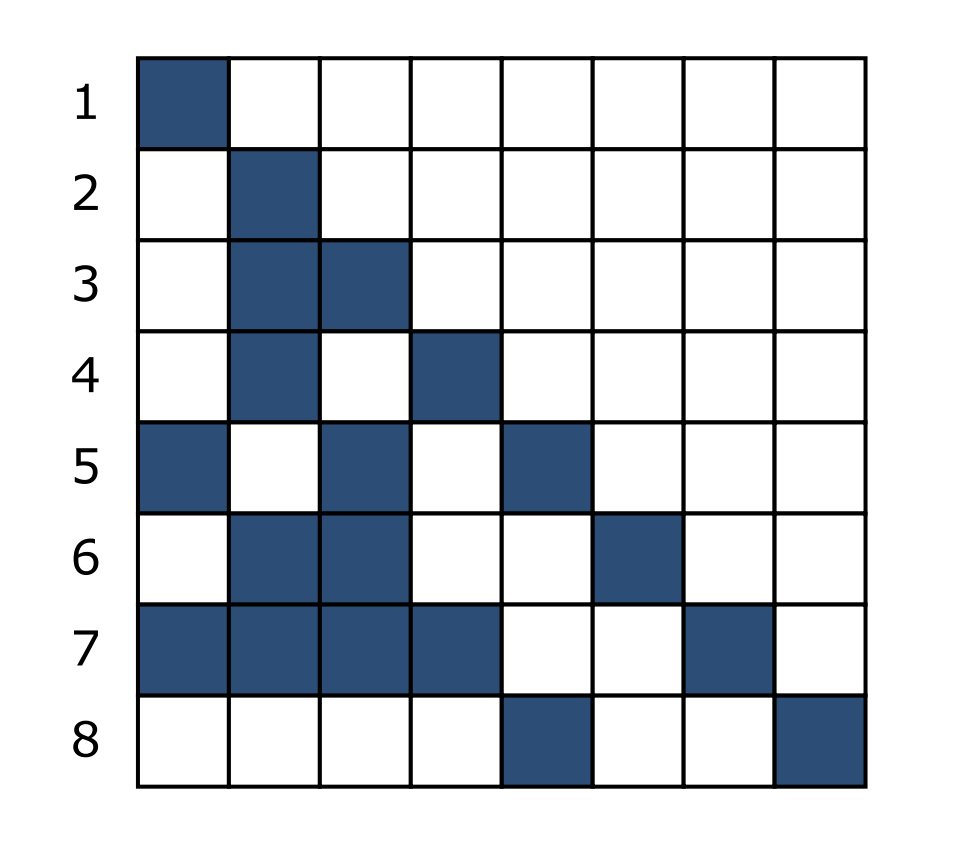
\includegraphics[width=.8\linewidth]{report/figures/lr_2_2_ex_1.png}
  \caption{}
\end{subfigure}%
\begin{subfigure}{.5\textwidth}
  \centering
  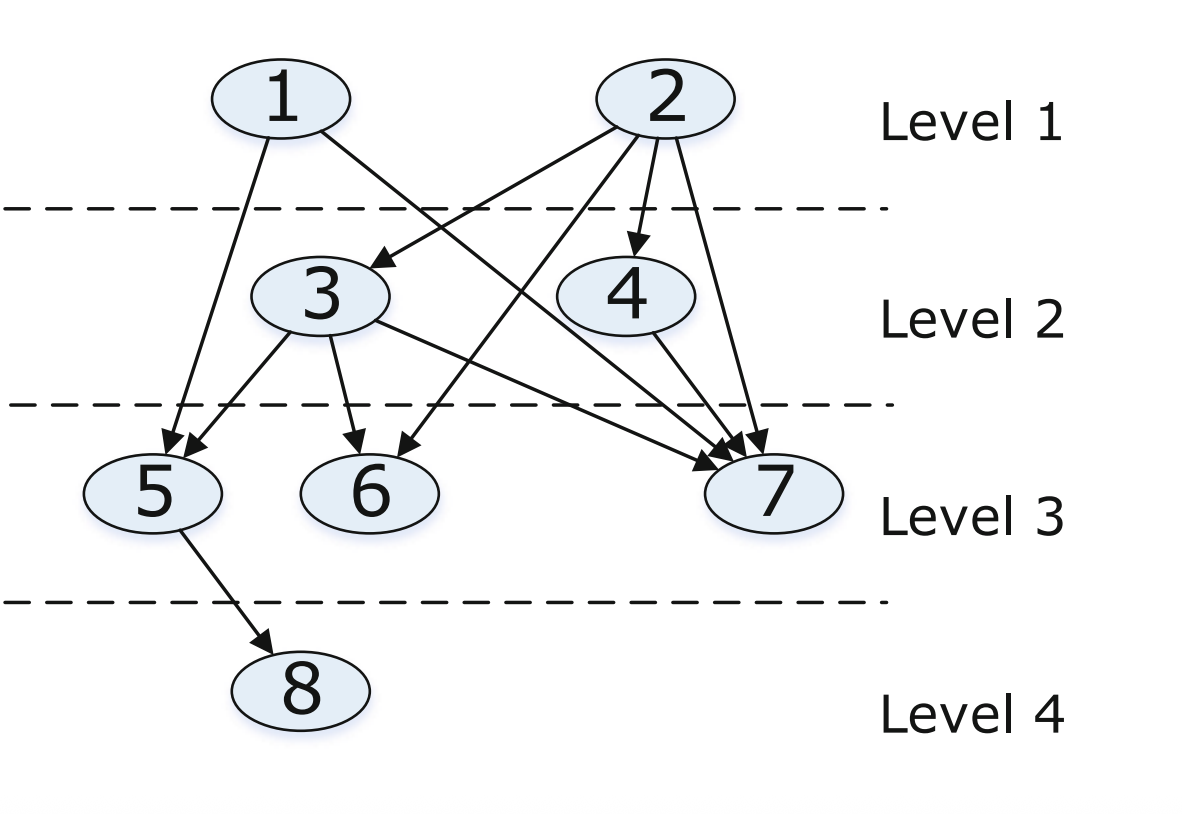
\includegraphics[width=.8\linewidth]{report/figures/lr_2_2_ex_2.png}
  \caption{}
\end{subfigure}
\caption{(a) Non-zero pattern of a lower
triangular sparse matrix and (b) its corresponding task dependency graph of forward solver with level annotations \cite{10.1007/978-3-319-07518-1_8}}
\label{fig:example_lr_2_2}
\end{figure}

\subsection{Challenges Arising from Dependency Graphs}
While the DAG view of a sparse triangular system enables the identification of parallelism, it also highlights several challenges. First, the depth of the dependency graph, which corresponds to the length of the critical path, ultimately limits the degree of parallelism that can be exploited \cite{10.1007/978-3-319-07518-1_8}. 

Second, the irregularity of the sparsity pattern leads to non-uniform workloads across parallel threads. Some rows may become ready to compute sooner than others, causing load imbalance. Managing these dynamic dependencies efficiently requires intelligent scheduling strategies, often using techniques such as level scheduling, graph colouring, or block-based decomposition \cite{10.1007/978-3-031-64850-2_42}.

Third, traversing a sparse matrix produces irregular, non-contiguous memory accesses.  Besides lowering cache hit rates, two threads may unknowingly touch different elements that reside in the same 64-byte cache line. If one of them writes, the line must be passed back and forth between their private caches (a phenomenon called false sharing), adding extra cache-level synchronisation even in
the absence of true data conflicts \cite{data_layout}.

Thus, while sparsity makes parallelism possible, achieving high performance in practice requires addressing these architectural and algorithmic challenges. The remainder of this thesis focuses on methods that mitigate these challenges.

% Technical Background
\section{Parallelization}
\label{chap:lr_technical_background}
The efficient solution of sparse triangular linear systems is not only a question of numerical methods, but also heavily depends on the characteristics of modern computer architectures. To understand the performance challenges and design choices in sparse triangular solvers, it is essential to consider how data is stored, moved, and processed at the hardware level. This section provides a brief overview of the relevant concepts in computer organization and parallel computing that are necessary to understand the techniques explored in this thesis.

\subsection{Memory Hierarchy and Cache Efficiency}
When solving large systems of equations numerically, a common misconception is that the computational speed of the processor (measured in FLOPs, or floating-point operations per second) is the main limiting factor. In reality, especially for sparse problems, the primary bottleneck often lies in memory access.

To mitigate this, processors use a hierarchy of caches (L1, L2, L3), which are small but fast memory units located closer to the CPU cores. Accessing data from L1 cache can be around 100× faster than accessing it from main memory \cite{levinthal2010performance}. Consequently, algorithms that reuse data in cache (temporal locality) and access data in a way that aligns with cache-friendly patterns (exploiting spatial locality) are significantly faster in practice.

Sparse triangular solvers, however, face a unique challenge: the matrix data is sparse, meaning it contains mostly zero entries, and is typically stored in a compressed format. This leads to indirect memory accesses through index arrays, causing irregular and often unpredictable access patterns. Such irregularity makes it difficult to exploit cache locality, resulting in frequent cache misses and wasted computational resources.

For these reasons, improving cache efficiency becomes more important than reducing the number of arithmetic operations. Techniques like blocking (dividing the matrix into small sub-matrices, or blocks, that fit into cache) and matrix reordering aim to improve data locality, reducing cache misses during the solve phase.

\subsection{Instruction-Level and Thread-Level Parallelism}
While individual CPU cores have become only marginally faster over the last decade, overall computational capacity has increased through parallelism. Modern processors feature multiple cores that can operate simultaneously, allowing multiple operations to proceed in parallel. Modern CPUs can exploit multiple forms of parallelism which are discussed here below.

Instruction-Level Parallelism (ILP): Within a single core, multiple instructions can be processed in parallel through pipelining and superscalar execution. However, ILP is largely automatic and limited by data dependencies; It does not suffice to accelerate algorithms like sparse triangular solves, where computations often depend on results from earlier steps \cite{rauber2023parallel}.

Thread-Level Parallelism (TLP): This refers to running multiple threads of execution across multiple CPU cores. Threads can operate on independent data or different parts of a problem simultaneously. For instance, if two parts of a matrix can be processed independently, they can be assigned to different threads, leveraging the parallelism of the hardware \cite{rauber2023parallel}.

\subsection{Task Parallelism and Dependency Management}
Sparse triangular solves require fine-grained and irregular parallelism. Here, the concept of task parallelism becomes useful.

In task-based parallelism, the problem is divided into discrete units of work called tasks. Tasks can be thought of as mini-programs that perform a specific computation (e.g., solving for a block of unknowns in a triangular solve). These tasks can be executed concurrently, as long as data dependencies are respected.

Modern parallel programming frameworks like OpenMP provide constructs to express such task dependencies explicitly. For instance, OpenMP 4.5 and later versions allow developers to annotate tasks with depend clauses, specifying which data is read and written by each task \cite{openmp2015programminginterface}. The runtime system then schedules tasks dynamically, ensuring correctness while trying to maximize concurrency.

In the context of sparse triangular solvers, we can express the solution process as a Directed Acyclic Graph (DAG), where nodes represent computational tasks (e.g., solving a block of unknowns) and edges represent data dependencies between these tasks.
The DAG-based task scheduling enables the solver to overlap independent computations, making effective use of multiple threads. It also allows for redundant computations where beneficial, trading extra arithmetic for better cache reuse and parallel efficiency.

% Current methodes
\section{Existing Methods}
\label{chap:lr_current_methodes}
Over the years, a variety of methods and optimizations have been proposed to address the issues mentioned in the previous sections. In this section, we provide an overview of the most relevant approaches and introduce the widely used libraries against which we will benchmark our own method.

\subsection{Level Scheduling}
One of the earliest and most widely adopted strategies for parallel sparse triangular solves is level scheduling. The idea is to preprocess the matrix to identify sets of unknowns that can be solved independently because they do not depend on each other. These sets are called levels. Solving proceeds level by level, with all unknowns within a level computed in parallel, followed by a global barrier that ensures every thread has finished that level before the next one can begin.

While straightforward, level scheduling is limited in its effectiveness because the number of available levels often grows logarithmically with the problem size, resulting in limited parallelism for large sparse systems. Moreover, extracting levels adds preprocessing overhead, and the benefit depends heavily on the sparsity structure of the matrix \cite{10.1007/978-3-031-64850-2_42}.

\subsection{Blocked and Supernodal Methods}
A different strand of work targets blocked or supernodal representations. During the factorisation step these approaches
group contiguous columns whose non-zero patterns are identical (supernodes) so that the expensive updates can be cast as dense
matrix–matrix multiplies and handled by highly-tuned BLAS Level-3
kernels. In the subsequent triangular solve phase each supernode
is treated as a dense triangular block, which reduces indirect indexing
and improves cache reuse, although the per-block operation is now a
matrix–vector multiply (BLAS Level-2) and therefore still memory-bound.

Supernodal techniques pay off when the matrix contains large, regular
blocks. For matrices that remain highly irregular the gains taper off, and additional fine-grained
parallel strategies become necessary \cite{10.1145/3404397.3404428}.

\subsection{Dependency Graph Approaches and Task Parallelism}
More recently, methods based on dependency graphs and task-based parallelism have gained prominence. Instead of grouping unknowns into coarse-grained levels, these approaches represent the triangular solve as a Directed Acyclic Graph (DAG) of fine-grained tasks, with edges representing data dependencies  \cite{10.1007/978-3-031-64850-2_42}.

Frameworks like OpenMP tasking and Kokkos task DAGs allow expressing these dependencies explicitly. The runtime system dynamically schedules tasks while respecting data dependencies, enabling finer granularity of parallelism and better utilization of modern multicore processors.

These DAG-based approaches can adapt to highly irregular sparsity patterns and allow advanced strategies like redundant computations and asynchronous execution, which can improve both cache locality and load balancing across cores.

\subsection{Specialized Sparse Triangular Solvers in Libraries}
Several mature HPC libraries ship hand-tuned sparse-triangular kernels.  
On CPUs the best-known package is the Intel Math Kernel Library (Intel MKL).  
Its sparse BLAS call \texttt{mkl\_sparse\_d\_trsv} is aggressively vectorised and cache-aware, yet the actual forward or backward substitution still executes on a single OpenMP thread.  
Because the code base is highly optimised, this serial kernel often rivals or exceeds naïve threaded versions and therefore remains a good baseline for CPU studies \cite{carvalho2015performance}.  
In the present work MKL serves as a reference for what can be achieved with one core and near-optimal data locality.

To place the new solver in a genuinely parallel context the experiments also use KokkosKernels, the task-DAG backend of the Kokkos ecosystem.  Its \texttt{sptrsv\_symbolic/solve} pair offers several level-scheduling algorithms that exploit nested parallelism on multicore CPUs and GPUs while remaining fully open source and architecture agnostic.  
Kokkos therefore represents the current state of portable, task-parallel techniques aimed at shared-memory machines.

Packages such as cuSPARSE for NVIDIA GPUs, the Ifpack2/Tpetra modules inside Trilinos, or the classical Hypre library also provide SpTRSV routines, but they are not benchmarked here.  
The proposed algorithm is tailored to cache-based shared-memory CPUs, and Kokkos already embodies the modern parallel strategies that those other libraries increasingly adopt.

The performance study thus compares three solvers: the serial but highly tuned MKL routine, the fully parallel implementation from KokkosKernels, and the method introduced in this thesis.  In Chapter \ref{chap:implementation} these libraries will be discussed in greater detail.

% Motivation for our approach
\section{Motivation for Our Approach}
\label{chap:lr_motivation}
While existing SpTRSV methods and libraries offer a range of techniques to address the challenges posed by sparsity and parallelism, they often involve trade-offs between generality, scalability, and memory efficiency. Level scheduling is constrained by limited parallelism, supernodal methods require favourable matrix structures to be effective, and task-based runtimes still face difficulty in balancing overhead with computational benefit, especially for fine-grained tasks. Moreover, many existing solvers are designed to perform optimally on matrices with specific sparsity patterns or hardware characteristics, limiting their general applicability. In contrast, the method proposed in this thesis is motivated by the need for a sparse triangular solver that is both cache-efficient and well-suited to shared-memory parallel architectures, especially in the context of very large systems where such considerations have a measurable impact on performance. By using redundant computation, block decomposition, and task parallelism, the proposed approach seeks to exploit both structural and hardware-level opportunities for concurrency that are often underutilized in conventional solvers.

